\documentclass{article}

%Headers
\usepackage[dvips]{graphicx}    %package that does pdfs
\usepackage{color}              %this needs to be here also

\title{CS440: The Maze is on Fire}
\author{Andy Rivera, John Juarez}
\date{February 19, 2021}

\begin{document}
\maketitle

\section{Maze Generation and Project Setup}
   To generate a maze we used the function \textbf{generateMaze(int dim,double p)} it takes in the parameters of  \textit{dim} to construct a dimxdim 2D array and \textit{p} to determine the probability of a block being filled(1) or not(0).
   
   To set up the project for the path finding algorithms we created an object \textbf{Point} with the following attributes:
   \begin{itemize}
   \item Point parent (Previous location of agent)
   \item X and Y to keep track of location of agent
   \item stepsTaken (Amount of steps taken to get to the current location.)
   \item Hueristics (Estimate for A* algorithm)
   \end{itemize}

\begin{figure}[hpt]

\centering
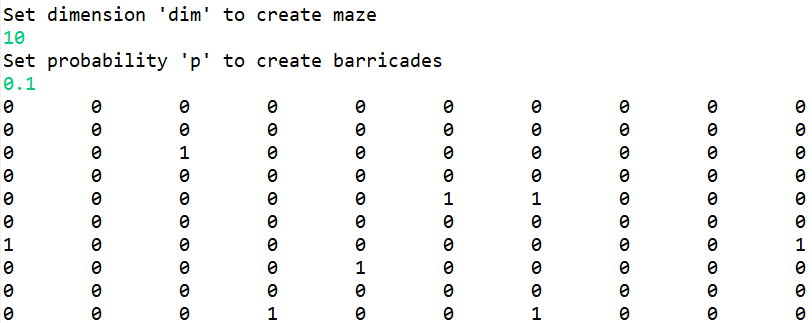
\includegraphics[width=3.5in]{maze1}\hfill
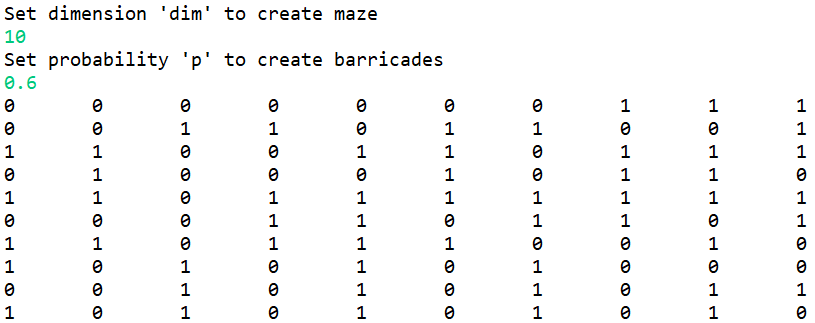
\includegraphics[width=3.5in]{maze3}

\caption{Maps generated with p = 0.1 and 0.6 respectively}
\label{fig:figure1}

\end{figure}


\section{DFS Algorithm}
 We created the method \textbf{mazeDFS(int[][] maze, Point start, Point goal).} It takes in 2 points and returns a boolean, True if there exists a path and false if no path exists between the starting point and the goal point. 
	
	With two arbitrary points in the maze, DFS would be a better option because we are just determining if there is a path between the two points and not necessarily the shortest path, it will save space in memory since it adds less points into the fringe by not exploring all of its neighbors.
	\begin{figure}[hbt!]

\centering
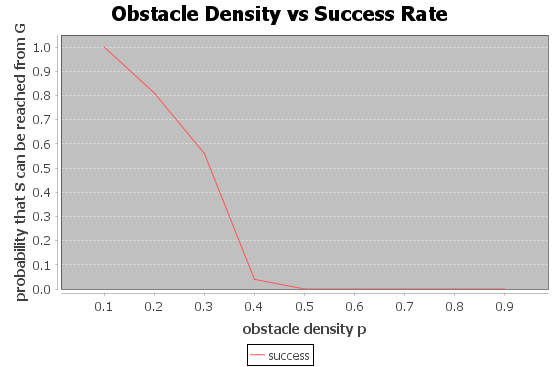
\includegraphics[width=3.5in]{DFSanalysis}

\caption{obstacle density p vs probability that S can be reached from G}
\label{fig:figure2}

\end{figure}

\section{BFS and A* Algorithms}
   For our BFS algorithm, we created the method \textbf{mazeBFS(int[][] maze).} It returns the ArrayList of the points that make up the shortest path.
   
   For our A* algorithm, we created the method \textbf{mazeAStar(int[][] maze).} It uses a priority queue that prioritizes points based on an estimation that is determined by adding up the amount of steps taken(cost so far) + euclidean distance + the de-prioritization(Steps to the left and steps up will have less priority) of steps that take you further from goal.
   
   If there is no path between the starting point and the goal point the difference between nodes explored by BFS and A* would be 0 because both algorithms would keep trying to explore every point in the maze.                                                     
   
   \begin{figure}[hpt]
   \centering
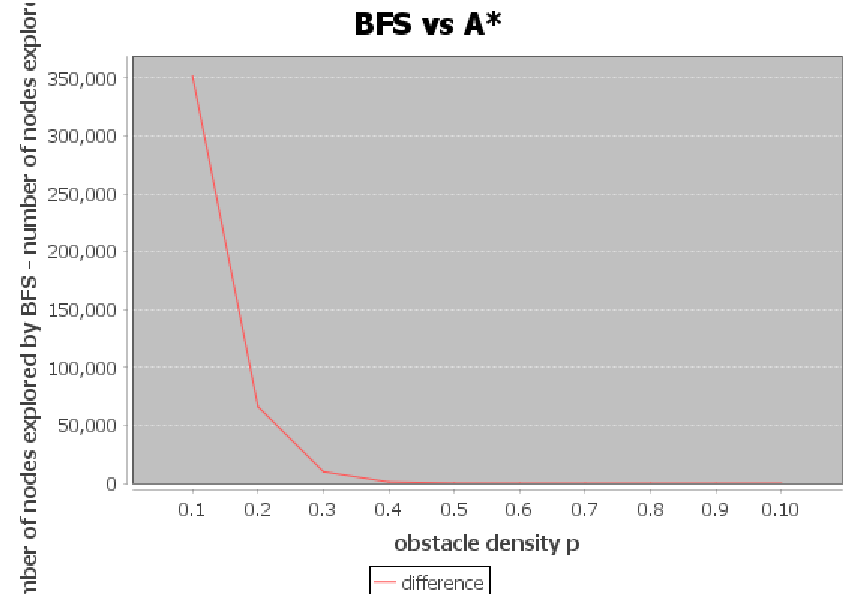
\includegraphics[width=3.5in]{BFSvA}

\caption{number of nodes explored by BFS - number of nodes explored by A* vs obstacle density p}
\label{fig:figure3}

\end{figure}
   
   \begin{figure}[hpt]
   \centering
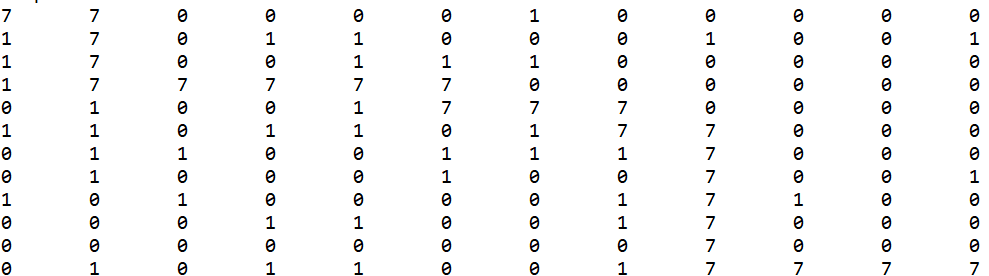
\includegraphics[width=3.5in]{BFS}

\caption{BFS Shortest path represented by 7 dim = 12 p = 0.3}
\label{fig:figure4}

\end{figure}

 \begin{figure}[hpt]
   \centering
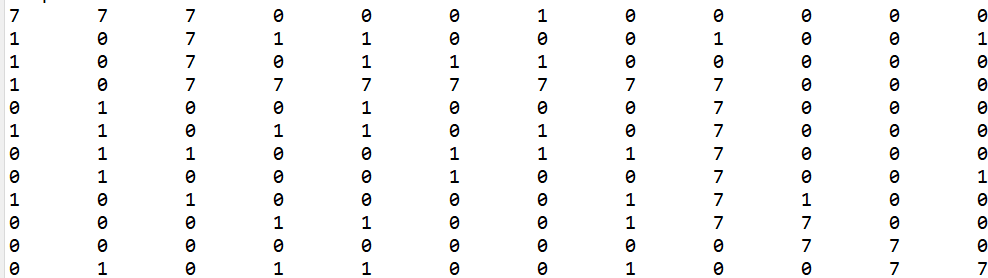
\includegraphics[width=3.5in]{astar}

\caption{A* Shortest path represented by 7 dim = 12 p = 0.3}
\label{fig:figure5}

\end{figure}

\bigskip
\bigskip

\section{Algorithms in less than 1 minute}	
At p = 0.3 the largest dimension size the algorithm can find a path in less than one minute is...
\begin{itemize}
\item \textbf{DFS} dim = 
\item \textbf{BFS} dim =
\item \textbf{A*}  dim =
\end{itemize}

\section{Strategy 3}
The strategy that we implemented finds an initial path from the starting point and the goal point. As the agent advances through the burning maze it also scans the path ahead before it advances. In a helper method \textbf{scanPath(int[][] maze, int currIndex, ArrayList<Point> path, ArrayList<Point> firePoints, double q)} it scans ahead of the agent by counting the steps of from the closest point that is on fire and determines the probability of the point catching on fire.

   The more burning neighbors the point has the greater the probability of the point catching fire next.  Using that as a threshold, if the point surpasses the threshold, the agent will try and generate a new path with less risk of catching on fire if there is one.  
   
   \begin{figure}[hpt]
   \centering
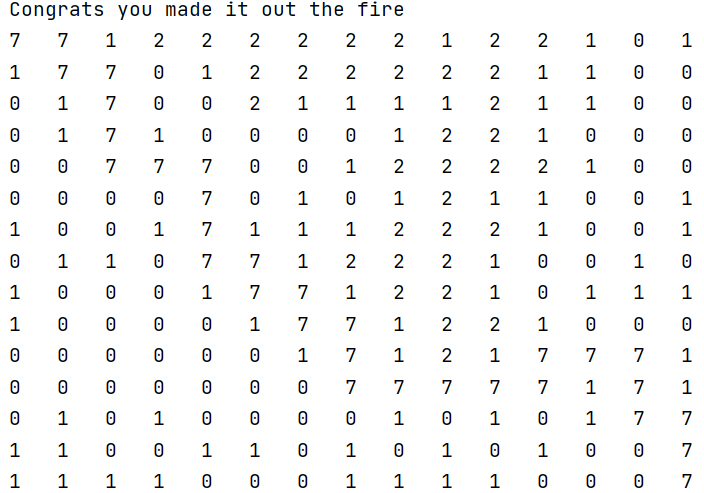
\includegraphics[width=3.5in]{strat3ex}

\caption{Strategy 3: dim = 15, p=0.3, q=0.3
7-represents path 2-represents fire}
\label{fig:figure6}
\end{figure}

\section{Strategies Success Rates}

\section{Unlimited Computational Resources}
	If we had unlimited computational resources, our strategy 3 would be able to scan and calculate the probability of all the points in the maze based on where the fire is starting and not only the initial path. Essentially adding all the points in the maze that are not on fire in it's fringe. It will almost always find a path since it can accurately predict all the points that are going to catch on fire and modifies it's path accordingly. 

\section{10 Seconds to Make a Move}
	
\end{document}